%%%%%%%%%%%%%%%%%%%%%%%%%%%%%%%%%%%%%%%%%
% Beamer Presentation
% LaTeX Template
% Version 1.0 (10/11/12)
%
% This template has been downloaded from:
% http://www.LaTeXTemplates.com
%
% License:
% CC BY-NC-SA 3.0 (http://creativecommons.org/licenses/by-nc-sa/3.0/)
%
%%%%%%%%%%%%%%%%%%%%%%%%%%%%%%%%%%%%%%%%%

%----------------------------------------------------------------------------------------
% PACKAGES AND THEMES
%----------------------------------------------------------------------------------------

\documentclass[table, xcolor={dvipsnames}, 9pt]{beamer}
\usepackage{tikz}
\usetikzlibrary{positioning}
\mode<presentation> {

% The Beamer class comes with a number of default slide themes
% which change the colors and layouts of slides. Below this is a list
% of all the themes, uncomment each in turn to see what they look like.

%\usetheme{default}
%\usetheme{AnnArbor}
%\usetheme{Antibes}
%\usetheme{Bergen}
%\usetheme{Berkeley}
%\usetheme{Berlin}
%\usetheme{Boadilla}
%\usetheme{CambridgeUS}
%\usetheme{Copenhagen}
%\usetheme{Darmstadt}
%\usetheme{Dresden}
%\usetheme{Frankfurt}
%\usetheme{Goettingen}
%\usetheme{Hannover}
%\usetheme{Ilmenau}
%\usetheme{JuanLesPins}
%\usetheme{Luebeck}
% \usetheme{Madrid}
\usetheme{metropolis}
%\usetheme{Malmoe}
%\usetheme{Marburg}
%\usetheme{Montpellier}
%\usetheme{PaloAlto}
%\usetheme{Pittsburgh}
%\usetheme{Rochester}
%\usetheme{Singapore}
%\usetheme{Szeged}
%\usetheme{Warsaw}

% As well as themes, the Beamer class has a number of color themes
% for any slide theme. Uncomment each of these in turn to see how it
% changes the colors of your current slide theme.

%\usecolortheme{albatross}
%\usecolortheme{beaver}
%\usecolortheme{beetle}
%\usecolortheme{crane}
%\usecolortheme{dolphin}
%\usecolortheme{dove}
%\usecolortheme{fly}
%\usecolortheme{lily}
%\usecolortheme{orchid}
%\usecolortheme{rose}
%\usecolortheme{seagull}
%\usecolortheme{seahorse}
%\usecolortheme{whale}
%\usecolortheme{wolverine}

%\setbeamertemplate{footline} % To remove the footer line in all slides uncomment this line
%\setbeamertemplate{footline}[page number] % To replace the footer line in all slides with a simple slide count uncomment this line

%\setbeamertemplate{navigation symbols}{} % To remove the navigation symbols from the bottom of all slides uncomment this line
}

\usepackage{graphicx} % Allows including images
\usepackage{booktabs} % Allows the use of \toprule, \midrule and \bottomrule in tables
\usepackage{multirow}
\usepackage{natbib}
\usepackage[]{hyperref}
\usepackage{diagbox}
\usepackage{makecell}
\usepackage{subfig}
\usepackage{amsmath}
\usepackage{amsfonts,amsthm,amsmath,amssymb}    
\usepackage{bbm}
\usepackage{bm}
\usepackage{empheq}

\hypersetup{unicode=true,
            pdfusetitle,
            bookmarks=true,
            bookmarksnumbered=true,
            bookmarksopen=true,
            bookmarksopenlevel=2,
            breaklinks=false,
            pdfborder={0 0 1},
            backref=true,
            hypertexnames=false,
            pdfstartview={XYZ null null 1}}
\usepackage{xcolor}
\newcommand\myheading[1]{%
  \par\bigskip
  {\Large\bfseries#1}\par\smallskip}
\newcommand\given[1][]{\:#1\vert\:}
\theoremstyle{newstyle}
\newtheorem{thm}{Theorem}
\newtheorem{prop}[thm]{Proposition}
\newtheorem{lem}{Lemma}
\newtheorem{cor}{Corollary}
\newtheorem{defin}{Definition}
\newcommand*\diff{\mathop{}\!\mathrm{d}}
\newcommand*\Diff[1]{\mathop{}\!\mathrm{d^#1}}
\newcommand*{\QEDA}{\hfill\ensuremath{\blacksquare}}%
\newcommand*{\QEDB}{\hfill\ensuremath{\square}}%
\DeclareMathOperator{\E}{\mathrm{E}}
\DeclareMathOperator{\R}{\mathbb{R}}
\DeclareMathOperator{\Var}{\rm{Var}}
\DeclareMathOperator{\Cov}{\rm{Cov}}
\DeclareMathOperator{\e}{\rm{e}}
\DeclareMathOperator{\logit}{\rm{logit}}
\DeclareMathOperator{\indep}{{\perp\!\!\!\perp}}
%\DeclareMathOperator{\Pr}{\rm{Pr}}
\newenvironment{Column}[1][.5\linewidth]{\begin{column}{#1}}{\end{column}}
%----------------------------------------------------------------------------------------
% TITLE PAGE
%----------------------------------------------------------------------------------------

\title[]{Sharp null hypothesis testing} % The short title appears at the bottom of every slide, the full title is only on the title page

\author{Thomas Leavitt} % Your name
\institute[] % Your institution as it will appear on the bottom of every slide, may be shorthand to save space
{
% Your institution for the title page
\medskip
\textit{} % Your email address
}
\date{\today} % Date, can be changed to a custom date

\begin{document}

\begin{frame}
\titlepage % Print the title page as the first slide
\end{frame}

%\begin{frame}
%\frametitle{Overview} % Table of contents slide, comment this block out to remove it
%\tableofcontents % Throughout your presentation, if you choose to use \section{} and \subsection{} commands, these will automatically be printed on this slide as an overview of your presentation
%\end{frame}

%------------------------------------------------------------------------
% PRESENTATION SLIDES
%------------------------------------------------------------------------
\section{Introduction}
\begin{frame}{Sharp null hypothesis testing: Introduction}
\begin{itemize}
\item Yesterday we introduced hypothesis tests of weak causal hypotheses \pause 
\begin{itemize}
\item I.e., hypotheses about only the average of study units' individual causal effects \pause 
\end{itemize}
\item Today we will go over tests of sharp causal hypotheses that provide a complete specification of unit-level responses to the experiment under every possible random assignment \pause 
\item We will introduce the mechanics of such tests and then consider their formal statistical properties \pause 
\begin{itemize}
\item E.g., type I error probability and power 
\end{itemize}  
\end{itemize}
\end{frame}
%------------------------------------------------------------------------
\begin{frame}{Sharp null hypothesis testing: An example}
\begin{itemize}
\item Consider the Acorn GOTV experiment (Arceneaux, 2005): \pause 
\item[]
\item[]
\begin{center}
  \begin{tabular}{r|rr|rrr}
  \hline
 & GOTV? & vote03(\%)& $y_c$ & $y_t$ & $\tau$\\
  \hline
1 & 0 & 38 & 38 & ? & ?\\
$\vdots$& & & & & \\
13 & 0 & 19 & 19& ? & ?\\
14 & 0 & 34 & 34& ? & ?\\
15 & 1 & 49 & ?& 49 & ?\\
16 & 1 & 38 & ?& 38 & ?\\
$\vdots$& & & & & \\
28 & 1 & 29 & ?& 29 & ? \\
   \hline
\end{tabular}
\end{center}
\end{itemize}  
\end{frame}
%------------------------------------------------------------------------
\section{Models of effects}
\begin{frame}{A simple model of effects for the Acorn GOTV experiment}
\begin{itemize}
\item Recall that a \textit{potential outcome schedule} is a complete specification of unit-level responses to the experiment under every possible random assignment \pause 
\item We can test any causal hypothesis about a potential outcome schedule \pause 
\item One simple model is that the GOTV campaign increases voter turnout by $p$ percentage points per precinct \pause 
\item[]
\item[]
\begin{center}
  \begin{tabular}{r|rr|rrr}
  \hline
 & GOTV? & vote03(\%)& $y_c$ & $y_t$ & $\tau$\\
  \hline
1 & 0 & 38 & 38 & $38 + p$ & $p$ \\
$\vdots$& & & & & \\
13 & 0 & 19 & 19 & $19 + p$ & $p$ \\
14 & 0 & 34 & 34 & $34 + p$ & $p$ \\
15 & 1 & 49 & $49 - p$ & 49 & $p$ \\
16 & 1 & 38 & $38 - p$ & 38 & $p$ \\
$\vdots$& & & & & \\
28 & 1 & 29 & $29 - p$ & 29 & $p$ \\
   \hline
\end{tabular}
\end{center}
\end{itemize}
\end{frame}
%------------------------------------------------------------------------
\begin{frame}{The sharp null hypothesis of no effect}
\begin{itemize}
\item Fisher's sharp null hypothesis of no effect states that the individual treatment effect is $p = 0$ percentage points for all precincts \pause 
\item[]
\item[]
\begin{center}
  \begin{tabular}{r|rr|rrr}
  \hline
 & GOTV? & vote03(\%)& $y_c$ & $y_t$ & $\tau$\\
  \hline
1 & 0 & 38 & 38 & 38 & 0 \\
$\vdots$& & & & & \\
13 & 0 & 19 & 19 & 19 & 0 \\
14 & 0 & 34 & 34 & 34 & 0 \\
15 & 1 & 49 & 49 & 49 & 0 \\
16 & 1 & 38 & 38 & 38 & 0 \\
$\vdots$& & & & & \\
28 & 1 & 29 & 29 & 29 & 0 \\
   \hline
\end{tabular}
\end{center}
\end{itemize}
\end{frame}
%------------------------------------------------------------------------
\begin{frame}{The distribution of the test statistic under the sharp null of no effect}
\begin{itemize}
\item The null distribution of the test statistic under Fisher's sharp null hypothesis of no effect \pause 
\item We could exactly enumerate all $\binom{28}{14} = 1,123,264,800$ test statistics, but this is too computationally intensive \pause 
\item Instead, we randomly sample from the set of $\binom{28}{14}$ possible assignments \pause 
\item[]
\item[]
\begin{figure}[H]
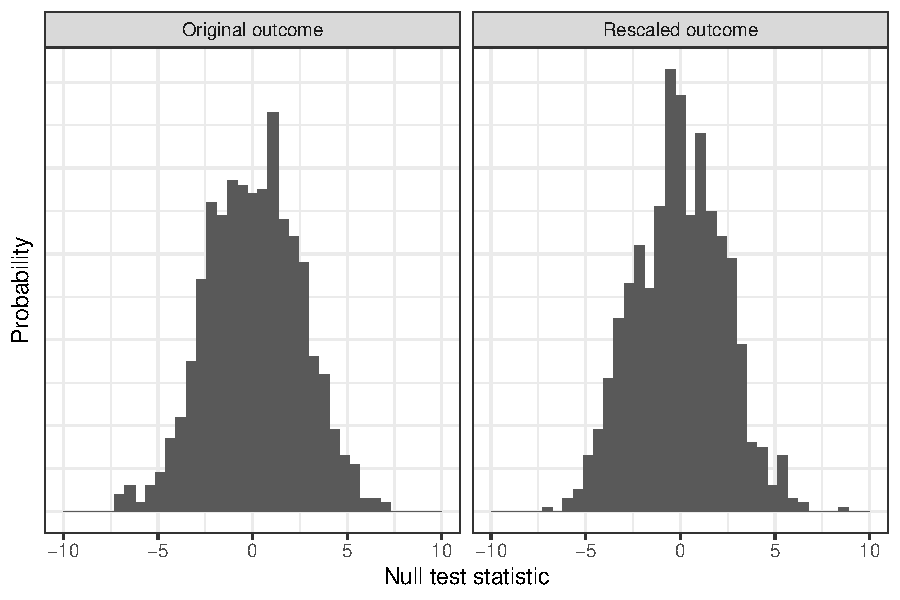
\includegraphics[width=0.7\linewidth]{null_dist_no_effect_plot.pdf}
\caption{Distribution of the Difference-in-Means test statistic under the sharp null of no effect}
\end{figure}
\end{itemize}
\end{frame}
%------------------------------------------------------------------------
\begin{frame}{Other sharp causal hypotheses}
\begin{itemize}
\item We need not test only the sharp null hypothesis that the individual effect is $0$ for all units \pause 
\item E.g., consider $p = 0.05$ for all $28$ precincts \pause 
\item[]
\end{itemize}
\begin{figure}[H]
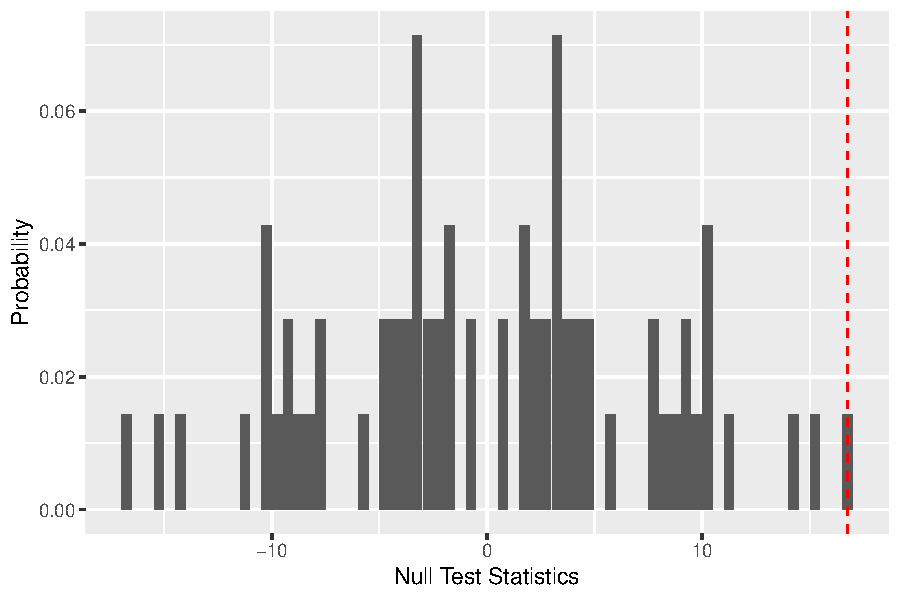
\includegraphics[width=0.7\linewidth]{null_dist_plot.pdf}
\caption{Distribution of the Difference-in-Means test statistic under the sharp null of $p = 0.05$ for all precincts}
\end{figure}
\end{frame}
%------------------------------------------------------------------------
\begin{frame}{Hypothesis tests via the uniformity trial}
\begin{itemize}
\item You can test a hypothesis specifying all of $\mathbf{y}_{c}$ even if it leaves blanks in $\mathbf{y}_{t}$ \pause 
\item \textit{Uniformity trial}:  Measure covariates, ``assign'' treatments $\mathbf{Z}$; but then don't administer any ($\mathbf{d}\equiv 0$). But measure outcomes anyway.  (Nowadays, a concept rather than a practice.) \pause 
\item An incomplete response schedule can still give us enough to do statistical testing. For example, if  \{hypothesis, $\mathbf{y}_{\mathrm{obs}}$\} together determine $\mathbf{y}_{U}$, the vector of responses that would have been obtained in the \textit{uniformity trial}, then for any test statistic $t $ we can test by comparing $t(\mathbf{z}, \mathbf{y}_{U})$ to the permutation distribution of $t(\mathbf{Z}, \mathbf{y}_{U})$
\end{itemize}
\end{frame}
%------------------------------------------------------------------------
\begin{frame}{Uniformity trial}
\begin{figure}[H]
\includegraphics[width=\linewidth]{null_plots.pdf}
\caption{Distributions of the Difference-in-Means test statistic under the sharp null hypotheses that $p = 0.05$ for all precincts}
\end{figure}
\end{frame}
%------------------------------------------------------------------------
\begin{frame}{Other sharp causal hypotheses}

\begin{center}
Let's go to \texttt{R} and test other sharp causal hypotheses . . . 
\end{center}

\end{frame}
%------------------------------------------------------------------------
\begin{frame}{Confidence sets and Hodges-Lehmann estimates} 
\begin{itemize}
\item A $1-\alpha$ confidence set for $p$ $\equiv $ \{$p$: $H_{p}$ not rejected at level $\alpha$\}
\item If you want an estimate to go with such a confidence interval, the convention is to report a \textit{Hodges-Lehmann} estimate ---
\begin{align*}
c: t\left(\mathbf{z}, \mathbf{y} - c\mathbf{Z}\right) & = \E\left[t\left(\mathbf{Z}, \mathbf{Y} - c\mathbf{Z}\right)\right]
\end{align*}
\item If there is no $c: t\left(\mathbf{z}, \mathbf{y} - c\mathbf{z}\right) = \E\left[t\left(\mathbf{Z}, \mathbf{Y} - c\mathbf{Z}\right)\right]$, then 
\footnotesize{\begin{align*}
\frac{1}{2} \sup \left\{c: \E\left[t\left(\mathbf{Z}, \mathbf{Y} - c\mathbf{Z}\right)\right] < t\left(\mathbf{z}, \mathbf{y} - c\mathbf{Z}\right)\right\}  + \frac{1}{2} \inf \left\{c: \E\left[t\left(\mathbf{Z}, \mathbf{Y} - c\mathbf{Z}\right)\right] > t\left(\mathbf{z}, \mathbf{y} - c\mathbf{Z}\right)\right\}
\end{align*}} \normalsize 
\end{itemize}
\end{frame}
%------------------------------------------------------------------------
\begin{frame}{Hodges-Lehmann estimates} 
\begin{figure}[H]
\includegraphics[width=\linewidth]{HL_null_dist_plot.pdf}
\caption{Distribution of the Difference-in-Means test statistic under the sharp null hypotheses that $p \approx 0.04$ for all precincts}
\end{figure}
\end{frame}
%------------------------------------------------------------------------
\section{Properties of sharp hypothesis tests}
\begin{frame}{Properties of sharp hypothesis tests}
\begin{itemize}
\item Type I error probability: Probability of rejecting the null when it is true is at least as small as $\alpha$ \pause 
\item Type II error probability: Probability of failing to reject the null when it is false  \pause 
\item Power: $1 - \text{Type II error probability}$; probability of rejecting null when it is false \pause 
\item Unbiased test: The probability of rejecting the null hypothesis when it is false and the alternative hypothesis is true is least as great as the probability of rejecting the null hypothesis when it is true and the alternative hypothesis is false (see Lehmann and Romano, 2005, chapter 4) \pause 
\item Consistent test: As the size of the study population increases asymptotically while all other relevant factors remain constant, the probability of rejecting the null hypothesis when it is false and the alternative is true should tend to 1 (see Lehmann and Romano, 2005, chapter 11).
\end{itemize}
\end{frame}
%------------------------------------------------------------------------
\begin{frame}{Properties of sharp hypothesis tests: Demonstration}
\begin{itemize}
\item Imagine that (unbeknownst to the researcher) the true causal effect for all $28$ precincts is $0.025$ \pause 
\item How would we assess the power to reject the sharp null hypothesis of no effect in favor of the alternative hypothesis of a positive effect? \pause 
\item Is the power of the test when the alternative is true at least as great as the type I error probability? \pause 
\item Let's do this in \texttt{R} . . . 
\end{itemize} 
\end{frame}
%------------------------------------------------------------------------
\end{document}